\documentclass[a4paper,12pt]{article}
\usepackage{a4wide}
\usepackage{tikz}
\usetikzlibrary{calc}

\begin{document}
\pagestyle{empty}
\setlength{\parindent}{0em}
\section*{RAM (Data Memory)}

Your task is to program the behavior of an entity called "RAM". This entity is declared in the attached file "RAM.vhdl" and has the following properties:
\begin{itemize}
\item Input:  Clk with type std\_logic
\item Input:  en\_read{{enReadIndex}} with type std\_logic
{{ENREAD}}\item Input:  en\_read2 with type std\_logic
\item Input:  en\_write{{enWriteIndex}} with type std\_logic
{{ENWRITE}}\item Input:  en\_write2 with type std\_logic
\item Input:  input{{inIndex}} with type std\_logic\_vector
{{IN2}}\item Input:  input2 with type std\_logic\_vector
\item Input:  addr1 with type std\_logic\_vector
\item Input:  addr2 with type std\_logic\_vector
\item Output: output{{outIndex}} with type std\_logic\_vector
{{OUT2}}\item Output: output2 with type std\_logic\_vector
\end{itemize}

\begin{center}
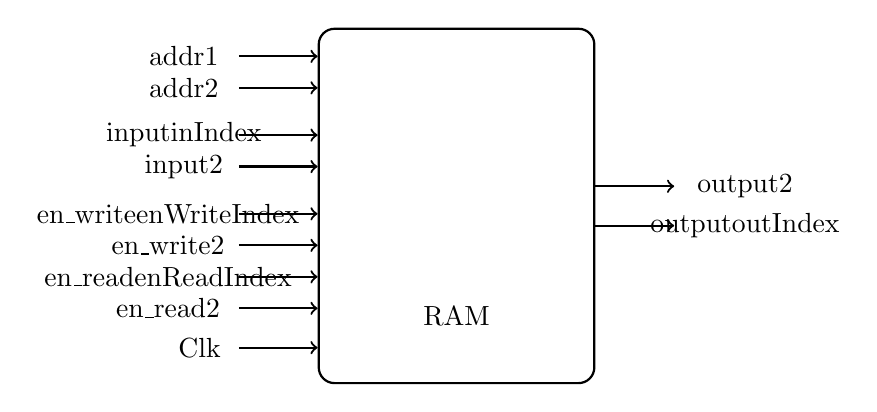
\begin{tikzpicture}
\draw node [draw,rectangle, minimum height=45mm, minimum width=35mm,rounded corners=2mm,thick](entity){};
\draw[->,thick] ($ (entity.west)-(10mm,18mm)$) -- ($ (entity.west) - (0mm,18mm)$);
\draw node at ($ (entity.west)-(15mm,18mm)$){Clk};

{{ENREAD}}\draw[->,thick] ($ (entity.west)-(10mm,13mm)$) -- ($ (entity.west) - (0mm,13mm)$);
{{ENREAD}}\draw node at ($ (entity.west)-(19mm,13mm)$){en\_read2};
\draw[->,thick] ($ (entity.west)-(10mm,9mm)$) -- ($ (entity.west) - (0mm,9mm)$);
\draw node at ($ (entity.west)-(19mm,9mm)$){en\_read{{enReadIndex}}};
{{ENWRITE}}\draw[->,thick] ($ (entity.west)-(10mm,5mm)$) -- ($ (entity.west) - (0mm,5mm)$);
{{ENWRITE}}\draw node at ($ (entity.west)-(19mm,5mm)$){en\_write2};
\draw[->,thick] ($ (entity.west)-(10mm,1mm)$) -- ($ (entity.west) - (0mm,1mm)$);
\draw node at ($ (entity.west)-(19mm,1mm)$){en\_write{{enWriteIndex}}};

{{IN2}}\draw[->,thick] ($ (entity.west)-(10mm,-5mm)$) -- ($ (entity.west) - (0mm,-5mm)$);
{{IN2}}\draw node at ($ (entity.west)-(17mm,-5mm)$){input2};
\draw[->,thick] ($ (entity.west)-(10mm,-9mm)$) -- ($ (entity.west) - (0mm,-9mm)$);
\draw node at ($ (entity.west)-(17mm,-9mm)$){input{{inIndex}}};

\draw[->,thick] ($ (entity.west)-(10mm,-15mm)$) -- ($ (entity.west) - (0mm,-15mm)$);
\draw node at ($ (entity.west)-(17mm,-15mm)$){addr2};
\draw[->,thick] ($ (entity.west)-(10mm,-19mm)$) -- ($ (entity.west) - (0mm,-19mm)$);
\draw node at ($ (entity.west)-(17mm,-19mm)$){addr1};

\draw[->,thick] ($ (entity.east) + (0mm,-2.5mm)$) -- ($ (entity.east) + (10mm,-2.5mm)$);
\draw node at ($ (entity.east) + (19mm,-2.5mm)$){output{{outIndex}}};
{{OUT2}}\draw[->,thick] ($ (entity.east) + (0mm,2.5mm)$) -- ($ (entity.east) + (10mm,2.5mm)$);
{{OUT2}}\draw node at ($ (entity.east) + (19mm,2.5mm)$){output2};

\draw node at ($ (entity) - (0,14mm)$){RAM};

\end{tikzpicture}
\end{center}

Do not change the file "RAM.vhdl".
\\

The "RAM" entity shall behave according to the following:
\\

Outputs of the entity and also the content of the RAM can only change on rising edges of the clock signal. The initial content of the memory is zero.\\
The address of a memory location, that the data is going to be written to or read from, is located on the address lines. When the reading or writing enables are active ('1'), the processes of reading or writing are performed on rising edges of the clock signal.

\begin{itemize}
{{Desc0}}\item The first address is the address of first writing operation (enabled with en\_write1) and also the reading operation (enabled with en\_read) and the second address is for the second writing operation (enabled with en\_write2) only.
{{Desc0}}\item When only en\_read is '1', the content of addr1 is read and put on the output.
{{Desc0}}\item When only en\_write1 is '1', input1 is written to addr1.
{{Desc0}}\item When only en\_write2 is '1', input2 is written to addr2.
{{Desc0}}\item Reading from addr1 and writing to addr2 can happen at the same time if addr1 is different from addr2{{RW22}}{{RW12}}{{RW21}}.
{{Desc0}}\item Two writing operations can happen at the same time if addr1 is different from addr2{{WW22}}.
{{Desc0}}\item Note that in any other cases, the content of the RAM must not be changed and the output shall be high impedance (Z).


{{Desc1}}\item The first address is the address of first reading operation (enabled with en\_read1) and also the writing operation (enabled with en\_write) and the second address is for the second reading operation (enabled with en\_read2) only.
{{Desc1}}\item When only en\_read1 is '1', the content of addr1 is read and put on output1.
{{Desc1}}\item When only en\_read2 is '1', the content of addr2 is read and put on output2.
{{Desc1}}\item When only en\_write is '1', input is written to addr1.
{{Desc1}}\item Reading from addr2 and writing to addr1 can happen at the same time only if addr1 is different from addr2{{WR22}}{{WR12}}{{WR21}}.
{{Desc1}}\item Two reading operations can happen at the same time.
{{Desc1}}\item Note that in any other cases, the content of the RAM must not be changed and the outputs shall be high impedance (Z).


{{Desc2}}\item The first address is the address of first reading operation (enabled with en\_read1) and also the first writing operation (enabled with en\_write1) and the second address is for the second reading (enabled with en\_read2) and writing operation (enabled with en\_write2) only.
{{Desc2}}\item When only en\_read1 is '1', the content of addr1 is read and put on output1.
{{Desc2}}\item When only en\_read2 is '1', the content of addr2 is read and put on output2.
{{Desc2}}\item When only en\_write1 is '1', input1 is written to addr1.
{{Desc2}}\item When only en\_write2 is '1', input2 is written to addr2.
{{Desc2}}\item Two writing operations can happen at the same time if addr1 is different from addr2{{WW22}}.
{{Desc2}}\item Reading from addr1 and writing to addr2 can happen at the same time if addr1 is different from addr2{{RW22}}{{RW12}}{{RW21}}.
{{Desc2}}\item Reading from addr2 and writing to addr1 can happen at the same time if addr1 is different from addr2{{WR22}}{{WR12}}{{WR21}}.
{{Desc2}}\item Two reading operations can happen at the same time.
{{Desc2}}\item Note that in any other cases, the content of the RAM must not be changed and the outputs shall be high impedance (Z).


{{Desc3}}\item The first address is the address of writing operation (enabled with en\_write) and the second address is for the reading operation (enabled with en\_read) only.
{{Desc3}}\item When only en\_write is '1', input is written to addr1.
{{Desc3}}\item When only en\_read is '1', the content of addr2 is read and put on the output.
{{Desc3}}\item Reading and writing operations can be done at the same time from/to the same address. Priority is with the reading operation which means that first the reading operation is done and then the writing operation.
{{Desc3}}\item Note that in any other cases, the content of the RAM must not be changed and the output shall be high impedance (Z).
\item When the memory is not read the related output shall be high impedance (Z).
\end{itemize}

 The length of the address is {{ADDRLENGTH}} bits, the length of input data {{WRITELENGTH}}, the length of output is {{READLENGTH}}, and the length of each memory cell is {{DATASIZE}} as well.
\begin{itemize}
{{Desc4}}\item When en\_write is active, the input data is written to the specified address. The length of the input is equal to the length of each memory cell.
{{Desc5}}\item The length of input is twice the length of each memory cell. Therefore, the lower half of the input should be written to the specified address and the upper half of the input should be written to the next higher address. We assume that the last memory address is never called for writing.
{{Desc6}}\item When en\_read is active, the data is read from the specified address. The length of the output is equal to the length of each memory cell.
{{Desc7}}\item The length of output is twice the length of each memory cell. Therefore, the content of specified address is read and put in the lower half of the output and the content of next higher address is read and transferred to the upper half of output. We assume that the last memory address is never called for reading.
\end{itemize}

This behavior has to be programmed in the attached file "RAM\_beh.vhdl".
\\

To turn in your solution, write an email to {{SUBMISSIONEMAIL}} with Subject "Result Task {{TASKNR}}" and attach your file "RAM\_beh.vhdl".

\vspace{0.7cm}
Good Luck and May the Force be with you.

\end{document}
\grid
